\documentclass[12pt]{article}
\usepackage{amsmath}
\usepackage{graphicx}
\usepackage{stmaryrd}

\author{Kyler Little}
\title{Homework \#2: Machine Learning}

\begin{document}
	\maketitle
	\section*{Problem \#1}
	(a) More generally, if we are learning from $\pm1$ data to predict a noisy target $P{y|\boldsymbol{x}}$ with candidate hypothesis $h$, show that the maximum likelihood method reduces to the task of finding $h$ that minimizes:
	\begin{equation}
	E_{\text{in}}(\boldsymbol{w})= \sum_{n=1}^{N} \llbracket y_n=+1\rrbracket \ln(\frac{1}{h(\boldsymbol{x}_n)}) + \llbracket y_n=-1\rrbracket \ln \frac{1}{1-h(\boldsymbol{x}_n)}
	\end{equation}
	(b) For the case $h(\boldsymbol{x}) = \theta (\boldsymbol{w}^T\boldsymbol{x})$, argue that minimizing the in-sample error in part (a) is equivalent to minimizing the one in (3.9).
	\\
	For two probabilistic distributions ${p, 1-p}$ and ${q, 1-q }$ with binary outcomes, the cross-entropy (from information theory) is:
	\begin{equation}
		p\log\frac{1}{q} + (1-p)\log\frac{1}{1-q}
	\end{equation}
	The in-sample error in part (a) corresponds to a cross-entropy error measure on the data point $(\boldsymbol{x}_n, y_n)$, with $p=\llbracket y_n=+1\rrbracket$ and $q=h(\boldsymbol{x}_n)$.
	\section*{Problem \#2}
	Recall the objective function for linear regression can be expressed as 
	\begin{equation}
	E(w) = \frac{1}{N} ||Xw-y||^2
	\end{equation}
	as in Equation (3.3) of LFD. Minimizing this function with respect to $w$ leads to the optimal
	$w$ as $(X T X)^{-1} X^T y$. This solution holds only when $X^TX$ is nonsingular. To overcome this problem, the following objective function is commonly minimized instead:
	\begin{equation}
	E_2(w) = ||Xw-y||^2 + \lambda ||w||^2
	\end{equation}
	where $\lambda > 0$ is a user-specified parameter. Please do the following: \\
	(a) Derive the optimal $w$ that minimize $E_2(w)$.\\
	(b) Explain how this new objective function can overcome the singularity problem
	of $X^T X$.
	
	\section*{Problem \#3}
	In logistic regression, the objective function can be written as:
	\begin{equation}
	E(w)=\frac{1}{N} \sum_{n=1}^{N} \ln(1+e^{-y_nw^Tx_n})
	\end{equation}
	(a) (10 points) Compute the first-order derivative $\nabla E(w)$. You will need to provide the intermediate steps of derivation.\\
	(b) (10 points) Once the optimal $w$ is obtained, it will be used to make predictions as follows:
	\begin{equation}
	\text{Predicted class of x} = 
	\begin{cases}
	1 & \text{if } \theta(w^Tx) \ge 0.5 \\
	-1 & \text{if } \theta(w^Tx) < 0.5 \\
	\end{cases}
	\end{equation}
	where the function $\theta(z) = \frac{1}{1+e^{-z}}$ looks like \\
	\begin{figure}[h]
		\begin{center}
			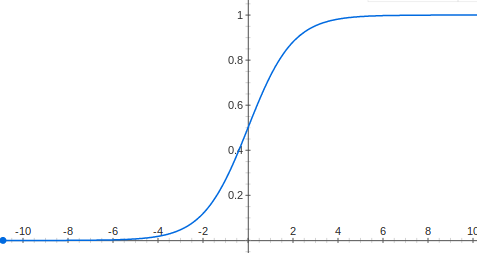
\includegraphics[width=3in]{sigmoid.png}
			\caption{A basic sigmoid curve}
			\label{fig:sigmoidEx}
		\end{center}
	\end{figure}
	\\ Explain why the decision boundary of logistic regression is still linear, though the linear signal $w^Tx$ is passed through a nonlinear function $\theta$ to compute the outcome of prediction.
	Is the decision boundary still linear if the prediction rule is changed to the following? Justify briefly.
	\begin{equation}
	\text{Predicted class of x} = 
	\begin{cases}
	1 & \text{if } \theta(w^Tx) \ge 0.9 \\
	-1 & \text{if } \theta(w^Tx) < 0.9 \\
	\end{cases}
	\end{equation}
	
	In light of your answers to the above two questions, what is the essential property of logistic regression that results in the linear decision boundary?
	
	\section*{Problem \#4}
	As your final deliverable to a customer, would you use the linear model with or without the 3rd order polynomial transform? Briefly explain your reasoning.
	
\end{document}